\chapter{Introduction}
\label{chap:introduction}

\section{Bilateria lineage}
Cerebral bilateral symmetry is a universal quality of organisms belonging to the Bilateria lineage \cite{Concha2012,Corballis2009}, the phylum incorporating all species with a single plane of symmetry, in contrast with their sister group, Cnidaria (\autoref{fig:bilateriaphylum}). Bilateral symmetry is a byproduct of the activity of two separate developmental processes, that produce two axes of polarity \cite{Finnerty2003}, and therefore a symmetry plane; the formation of a primary body axis, that corresponds to the long anatomical dimension of the animal, called \acf{rc} (i.e. head-to-tail), primarily dictated by highly conserved controlled activation of HOX genes during cell differentiation; the shaping of a secondary body axis, orthogonal to \ac{rc}, named \acf{dv} (i.e. back-to-front), attributed to a variety of genes,  such as the chromatin organizer CTCF, the left-right determination factor Nodal and central HOX genes \cite{Heger2020}. The remaining axis, \acf{lr}, is the one along which the symmetry pattern is manifested. On account of the high biodiversity that bilateria group includes, only the subgroup of vertebrates is examined in the following literature study. In addition, any reference to symmetry or asymmetry from now on corresponds to the \ac{lr} direction, unless explicitly mentioned.

This study makes an effort to statistically identify the genetic origins of a complex structural phenotype. Hence, examining, based on existing research, the main brain developmental stages is essential to discern the processes that induce bilateral symmetry. An important vertebrates (and bilateria) common characteristic is the germ line \textbf{triploblasticity}: the embryo begins as a flat disk, through a process called \textbf{gastrulation}, with three distinct cell layers; \textbf{endoderm}, \textbf{mesoderm}, and \textbf{ectoderm} \cite{F.Bear2016a}.  Of significance in the neural system formation is the ectoderm, which is initially equivalent to one of the flat disk sides. Under the context of this study, although a fact not directly connected to the brain cortex, it is necessary to mention that the perfect bilateral symmetry pattern appears to break even before gastrulation. In Xenopus (frog species) embryos, during fertilization and the initial 4-cell cleavage of the fertilized egg , the \textbf{cytoskeleton microtubules} appear to asymmetrically localize the ion channels proteins, whose \acs{rna} has been passed on by the mother, with a preference for the right side of the complex \cite{Aw2008}. Chicks embryos also exhibit a similar pattern. The occurrence of asymmetry at this extremely early time point underlines the significant role it has on the embryo development, species fitness, and, concomitantly, the conservation potential of this trait drivers \cite{Aw2009}. Another cellular component that is considered to enhance asymmetry, during gastrulation, is the motile cilia, hair-like organelles on the cell surface with the ability to beat \cite{Grimes2017}. Their movement is by construction asymmetric, causing a leftward flow of extraembryonic fluid and, subsequently, asymmetric distribution of exogenously introduced proteins \cite{Okada2005}. Both studied phenomena point to early initiation of asymmetric genes expression.

\begin{figure}
	\centering
	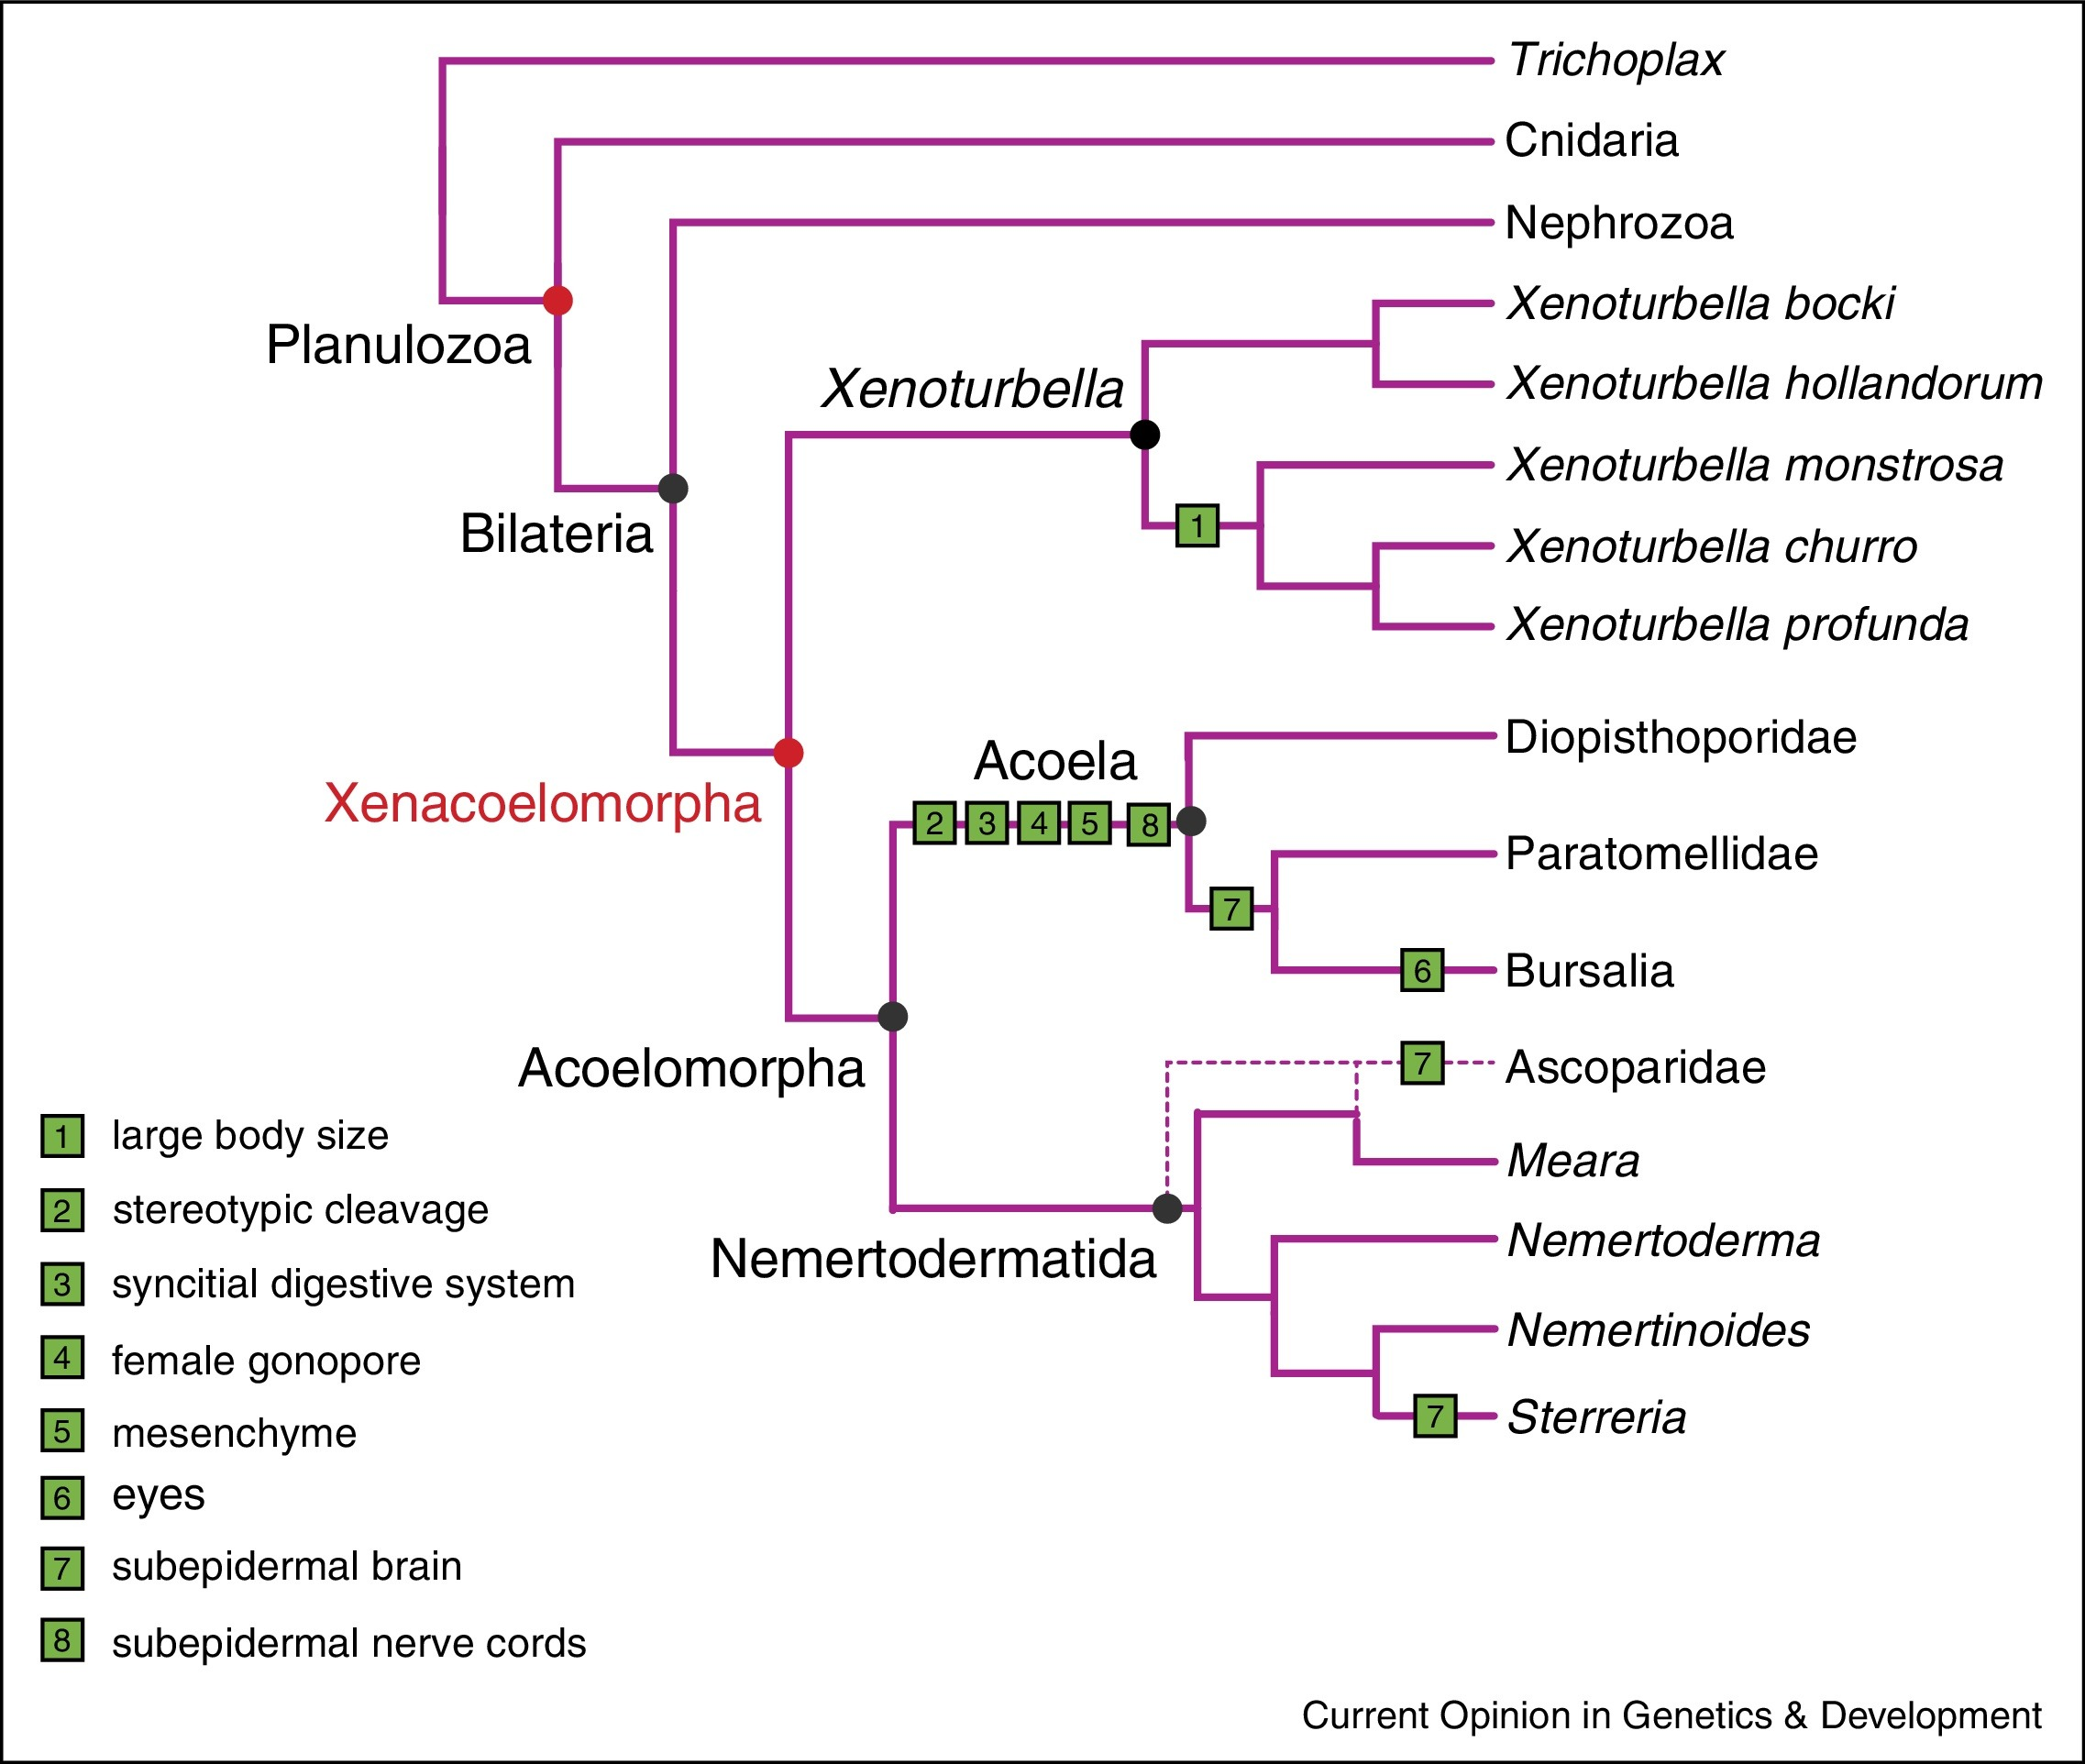
\includegraphics[width=0.9\linewidth]{bilateria_phylum}
	\caption[Bilateria clade \cite{Hejnol2016}]{Species phylogenetic tree subset, displaying bilateria clade, its sister clade, Cnidaria, and the direct children\cite{Hejnol2016}. Of great importance on the evolutionary studies of bilateral symmetry is the Xenacoelomorpha clade.}
	\label{fig:bilateriaphylum}
\end{figure}

\section{Symmetry during \acs{cns} formation}
Shortly after gastrulation, the disk folds, in a way that the central region of the ectoderm, called neural plate, forms a tube-like shape, the \textbf{neural tube}, which acts as the neural system precursor, under a process called \textbf{neurulation}. All bilateria have a \acf{cns}, which entirely develops from the neural tube walls \cite{F.Bear2016a}. The next pivotal step in the brain development, \textbf{differentiation}, leads to the creation of three distinct compartments along \ac{rc} axis, at the neural tube rostral end, the \textbf{prosencephalon} (forebrain), which develops into the brain cerebrum, the \textbf{mesencephalon} (midbrain), and the \textbf{rhombencephalon} (hindbrain), that is later attached to the spinal cord in vertebrates. For the subsequent mechanisms and terminology to be compatible with human cerebrum related literature, the focus is shifted on mammals phylum and, spatially, on the prosencephalon. The differentiation proceeds, with two pairs of lumps extruding symmetrically from the prosencephalon, the \textbf{telencephalic} vesicles, the predecessors of cerebral region, and the optic vesicles, the precursors of optic nerves and retinas, while the central remaining structure is called \textbf{diencephalon} \cite{F.Bear2016b}. The telencephalic vesicles continue to grow, expanding also caudally and in parallel with the diencephalon, gradually assuming the form of the two hemispheres, while a new pair of vesicles appears on the rostral part of the diencephalon, giving rise to the \textbf{olfactory bulbs}. The neural tube shape also reacts to the changes, forming four distinct \textbf{ventricles} along the neural tube, with two of them, named lateral ventricles, being mirrored inside each of the telencephalic vesicles. The earliest stage where asymmetry is noted in an anatomic level inside the human brain is during the end of the first trimester of gestation \cite{Abu-Rustum2013}. Specifically, the choroid plexus, a specialized cell network that lies inside the ventricles, attached to the diencephalon, and produces most of the \textbf{cerebrospinal fluid} in the \ac{cns},  develops asymmetrically in each lateral ventricle. The cerebrospinal fluid is of great value for the developing brain, as the main source of nourishment, waste removal and protection \cite{Telano2021}. Such an asymmetry manifestation in a macroscopic level, therefore, may be the progenitor of other forms of asymmetry at a later developmental stage \cite{Schmitz2019}, even at the brain surface. Cerebral bilateral symmetry therefore begins breaking down during fetal development, producing an asymmetric brain (\autoref{fig:brainlat}), and giving rise to partial functional disassociation, called \textbf{brain lateralization}. Lateralization becomes visible when examining organisms' behavior, with the most studied trait in humans being handedness and language \cite{Schmitz2019,Corballis2009}. To better understand why and how the inner functions are related with the external brain cortex development, the underlying cellular processes of \textbf{neurogenesis} and  \textbf{neuron migration}, active throughout differentiation, need to be identified, before introducing the reader to the anatomy of the fully grown brain. For this purpose, a further focus on primates phylum is needed, given the differences exhibited when comparing different mammals, such as rodents\cite{Molnar2019}.


\begin{figure}
	\centering
	\includesvg[width=0.9\textwidth]{da_visualization}\\
	\caption[Human cerebrum brain asymmetry]{Illustration of human cerebrum brain asymmetry. Normalized differences of the distances of landmarks from the center of mass of each averaged hemisphere surface. See \autoref{sec:phenotype_intro} for more details on the preprocessing.}
	\label{fig:brainlat}
\end{figure}

\section{Neurogenesis and Neuronal Migration}
The cells initially comprising the neural tube walls are named \acp{npc}, and exhibit similar properties with stem cells, that is limited multipotency (i.e. they can differentiate into multiple cell types) and limited self-renewing (i.e. they can divide symmetrically into new \acp{npc} a finite number of times), while also properties of epithelial cells, that is polarity (i.e. asymmetric cellular organization, with distinct basal and apical surfaces)  and attachment (i.e. junctions tightly connect adjacent cells) \cite{Gotz2005}. This cells array is contained between the basal and apical laminae, lipid membranes lateral to each other, with the apical lamina facing the neural tube lumen \cite{Aaku-Saraste1997}, and the cells being radially distributed. During anatomical differentiation, around the 7th gestational week in humans \cite{Nowakowski2016}, self-renewing is activated, leading to cells proliferation and \ac{cns} bilateral expansion, while attachment is hindered, gradually exchanging the \acp{npc} with \acp{rgc}, the fate-restricted progenitors of neurons, marking the initiation of \textbf{neurogenesis}\cite{Gotz2005}. A \ac{rgc} acts as the main building block of the brain, from which a single neuron or a neural progenitor, that later divides symmetrically in neurons, is generated. \Acp{rgc}' pivotal role does not end here. As it can be seen in \autoref{fig:rgc}, \acsp{rgc} are stretched during development, with processes connected to the surface of neural tube successor ventricles and to the outer cortical region surface, forming thread-like scaffolds. Newly formed neurons, generated from the \acsp{rgc} main, oval body, which remains close to the ventricles, use this structure as a guide to move towards the outer region of the cortex, under a process named \textbf{neuronal migration}\cite{Rakic2009}. This type of movement actually implies that the newly formed neurons head towards the brain surface, building the brain in an inside first, outside last fashion \cite{Molnar2019}. At later stages of human gestation, around week 19, studies have shown that a morphological transition is observed, where the majority of \acp{rgc} stops being attached to the \textbf{pial surface}, the outer surface of the brain, limiting the migration ability of neurons  \cite{Nowakowski2016} and affecting the way new layers are formed. Human neurogenesis extends to the third gestation trimester, being suppressed in case of premature birth \cite{Malik2013}. Postnatal neurogenesis is therefore presumed to be quite limited for primates \cite{Ernst2015}, despite the fact that the postnatal brain  dramatically increases in size , with that attributed to a rapid increase in neurons connections and glial cells (i.e. cells that provide physical and metabolic support to neurons) number \cite{Dyck2017}. The environmental factors that may affect brain symmetry are mainly detected before or during birth, with epigenetics and birth complications  appearing to be mostly correlated with handedness \cite{Schmitz2019,Cara2022}. In general, though, the more complex the phenomenon and the closer it is to humans, the higher the uncertainty and the greater the ethical restrictions. Only recently, non-invasive imaging and transcriptomic techniques have given further details regarding the brain development sequence, with genetic studies indirectly identifying the landscape of the underlying genes that affect different brain regions formation and symmetry \cite{Cara2022}. Moving on the literature study path and getting closer to the studied phenotype, the fully grown human brain cerebrum is subsequently anatomically described.

\begin{figure}
	\centering
	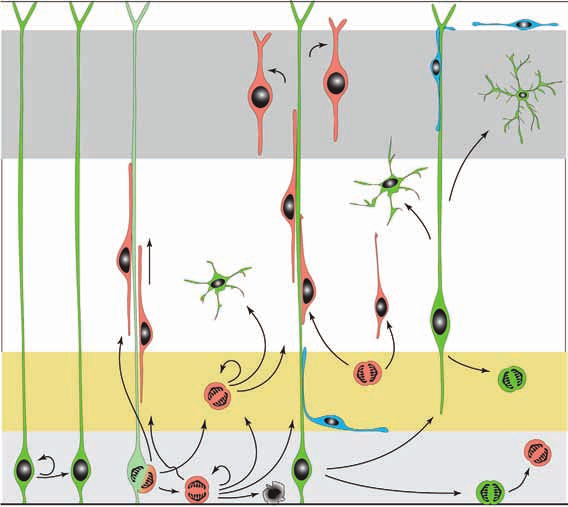
\includegraphics[width=0.8\textwidth]{rg_cells_division}\\
	\caption[A classical model of radial glial cells division processes \cite{Rakic2009}]{Illustration of a classical model of radial glial cells complex nonlinear division processes and neuronal migration \cite{Rakic2009}. From left to right: \acsp{npc} (green) originally divide symmetrically; During differentiation, \acsp{npc} become \acsp{rgc}, which divide asymmetrically, generating neurons or neural progenitor cells (orange). Neural progenitor cells eventually divide symmetrically into neurons. The majority of neurons in humans is produced by neuronal progenitors. A part of the generated neurons migrate radially towards the cortical plate, by attaching on the \acsp{rgc} projections; Eventually, after brain maturation, most \acsp{rgc} in humans undergo apoptosis (i.e. cell death) or generate neurons-supporting cells, such as astrocytes.}
	\label{fig:rgc}
\end{figure}


\section{The adult human cerebrum anatomic and functional properties}
 Human cerebrum is the center of sensations and thinking. The following excerpt provides a summarized anatomic and functional perspective, as described in the book of Bear et al. \cite{Bear2016chapter7app}, unless specified otherwise.  As aforementioned, cerebrum is entirely produced  from the telencephalon during fetal development, with the telencephalic vesicles ending up becoming the two hemispheres, that remain connected through what is known as the \textbf{Corpus callosum}.  The side view of each hemisphere is named \textbf{lateral}, and the view of the inner side is called \textbf{medial}. The human cerebrum outer covering surface is called \textbf{cerebral cortex}, the region on which the current study focuses. The human cerebrum appears distinctly different from other organisms, mainly due to the \textbf{sulci} (i.e. grooves) and \textbf{gyri} (i.e. bumps), with them being the result of the tremendous expansion of the cerebral cortex surface area during fetal development, folding and wrinkling in order to fit the skull. The precise pattern of gyri and sulci varies significantly across populations, rendering the brain surface unique per individual. Under a biopsy dissection or a \ac{mri} scan, the cerebrum appears to consist of two distinctly colored types of matter, implying changes in composition and consistency; the gray matter, at the outer part of the cerebrum, which  contains the cell bodies, dendrites and the axon terminals, where all synapses are, and the white matter, at the inner part, made up of myelinated (i.e. biologically insulated) axons, which connect different parts of gray matter to each other (\autoref{fig:cerebissection}). Protective layers on top of the gray matter, called \textbf{meninges}, ensure that the brain does not come in contact with the outer bone, with the one attached on and marking the outer borders of the gray matter named \textbf{pial surface}. In this study, the midthickness surface is examined, a term referring to the surface halfway between the pial and white matter surface. 

\begin{figure}[H]
	\centering
	\begin{subfigure}{0.475\linewidth}
		
		\centering
		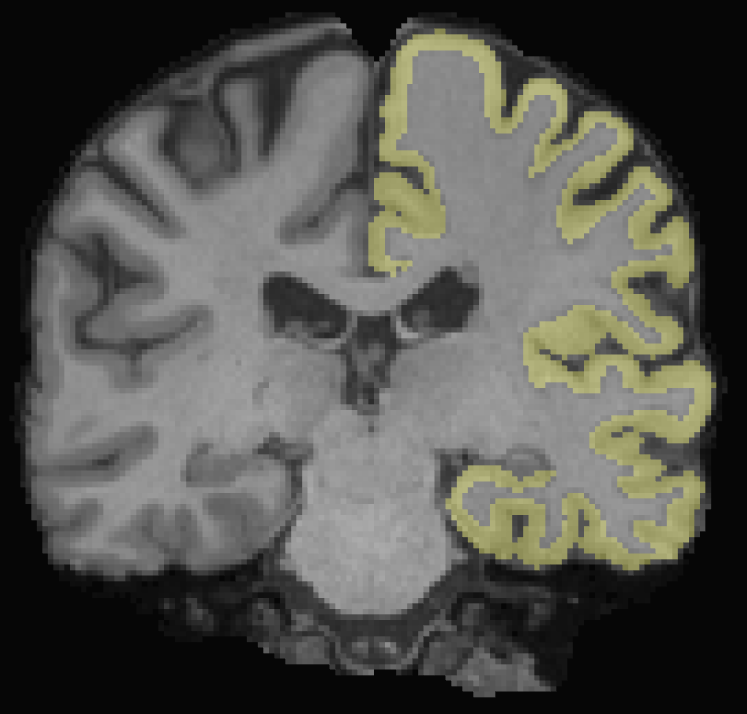
\includegraphics[width=0.475\linewidth]{coronal_section}
		\caption{Coronal section}
		\label{fig:coronal}
		
	\end{subfigure}
	\hfill
	\begin{subfigure}{0.475\linewidth}
		
		\centering
		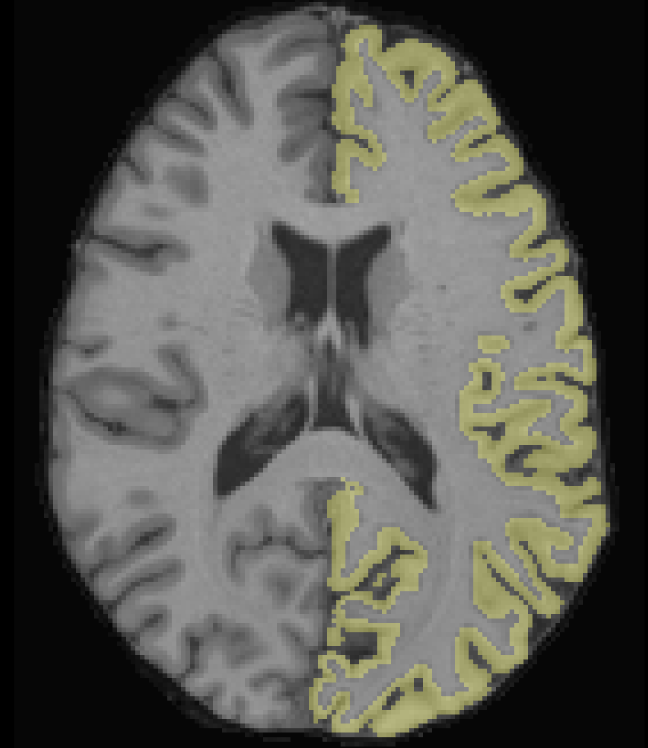
\includegraphics[width=0.475\linewidth]{axial_section}
		\caption{Axial section}
		\label{fig:axial}
	\end{subfigure}
	\vfill
	\begin{subfigure}{0.475\linewidth}
		
		\centering
		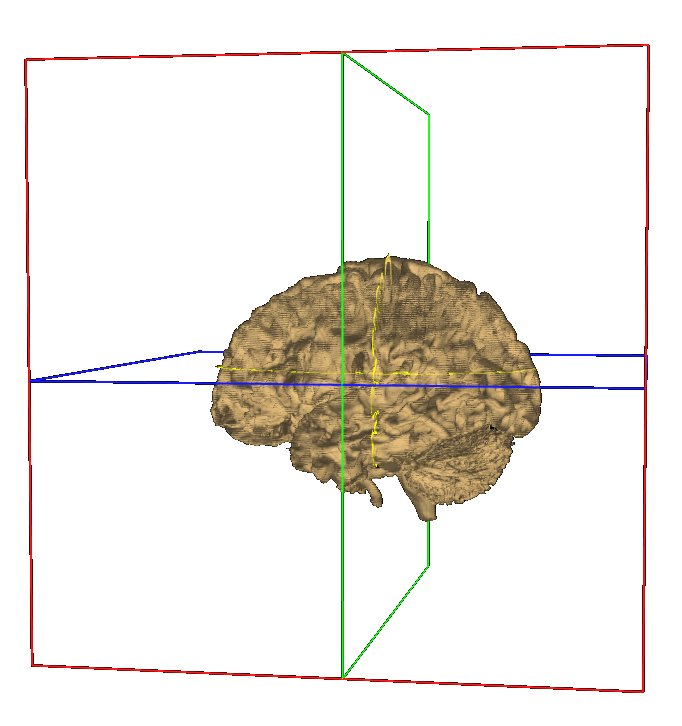
\includegraphics[width=0.475\linewidth]{3d_sections}
		\caption{\Ac{3d} sections map. Green rectangle corresponds to the coronal section plane (A) and
			blue rectangle to the axial section plane (B).}
	\end{subfigure}
	\caption[\Ac{mri} screening of gray and white matter]{Gray and white matter as seen from different sections, in an \ac{mri} screening, as retrieved from Freesurfer freeview routine. The gray matter is annotated with yellow color in the right hemisphere. Non brain regions have been removed.}
	\label{fig:cerebissection}
\end{figure}



\begin{figure}[H]
	\centering
	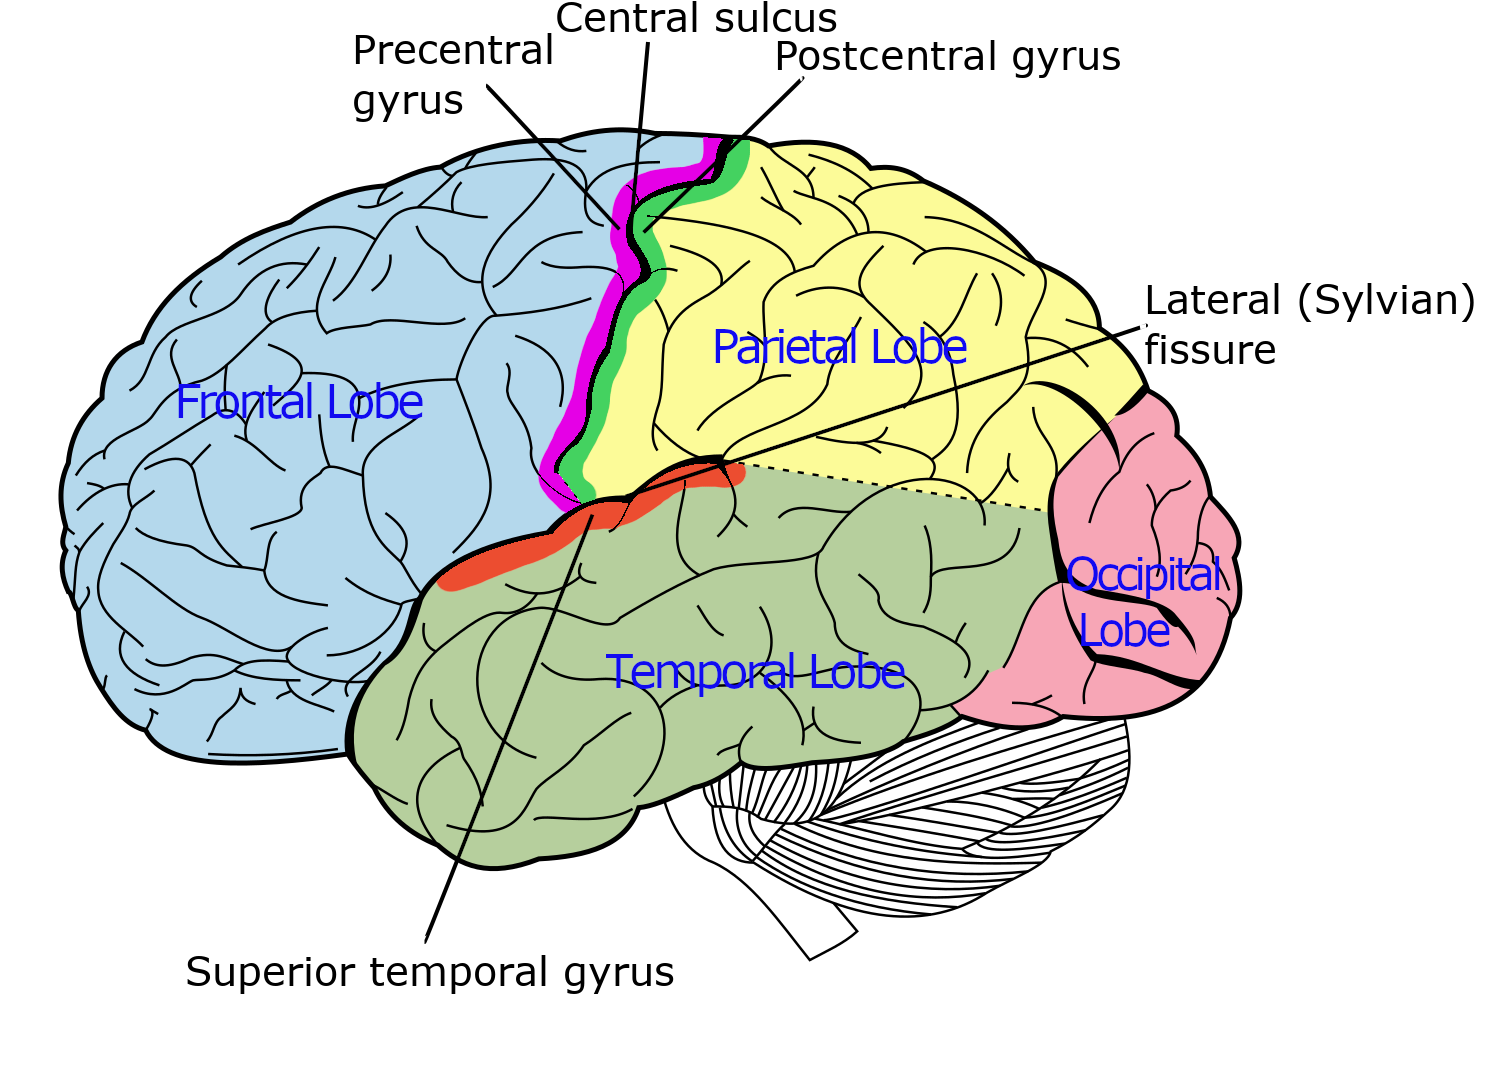
\includegraphics[width=0.8\textwidth]{1280px-Lobes_of_the_brain_NL.svg}
	\caption[A crude cerebrum partitioning]{Cerebrum lobes (blue font) and main gyri, sulci and fissures approximate positions (black font).}
	\label{fig:lobes}
\end{figure}

Efforts of partitioning the brain have been numerous throughout the years of medicine, with diverse resolution and purpose. Crudely, the cerebrum hemisphere is divided into lobes, that are named, by convention, after the bones of the skull that lie over them (\autoref{fig:lobes}).  A more detailed approach is based on the identification of the functional processes that take place in each part of the cortex, with Korbinian Brodmann being the first person constructing a 52-partitions experimentally based approximation of the hemisphere \cite{Brodmann1909} (\autoref{fig:corticalfunctions}). The main regions identified are:

\begin{figure}[H]
	\centering
	\centering
	\begin{subfigure}{0.475\linewidth}
		
		\centering
		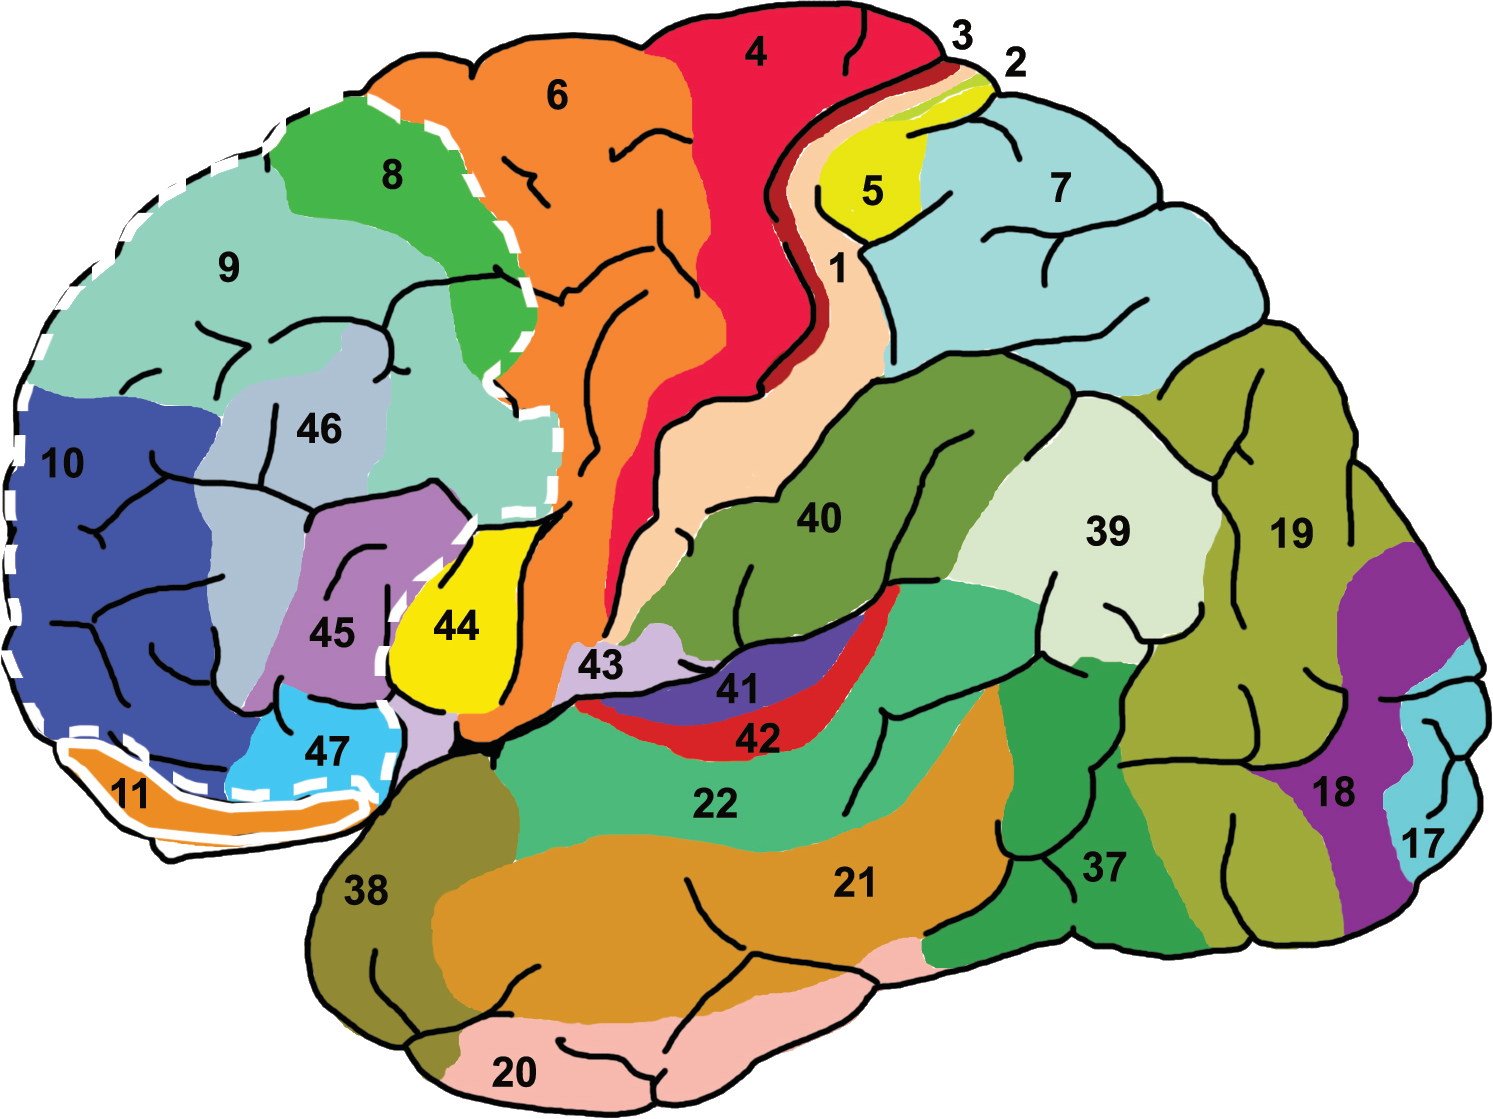
\includegraphics[width=0.8\linewidth]{brodmann_lateral}
		\caption{Lateral surface}
		\label{fig:brodmann_lateral}
		
	\end{subfigure}
	\hfill
	\begin{subfigure}{0.475\linewidth}
		
		\centering
		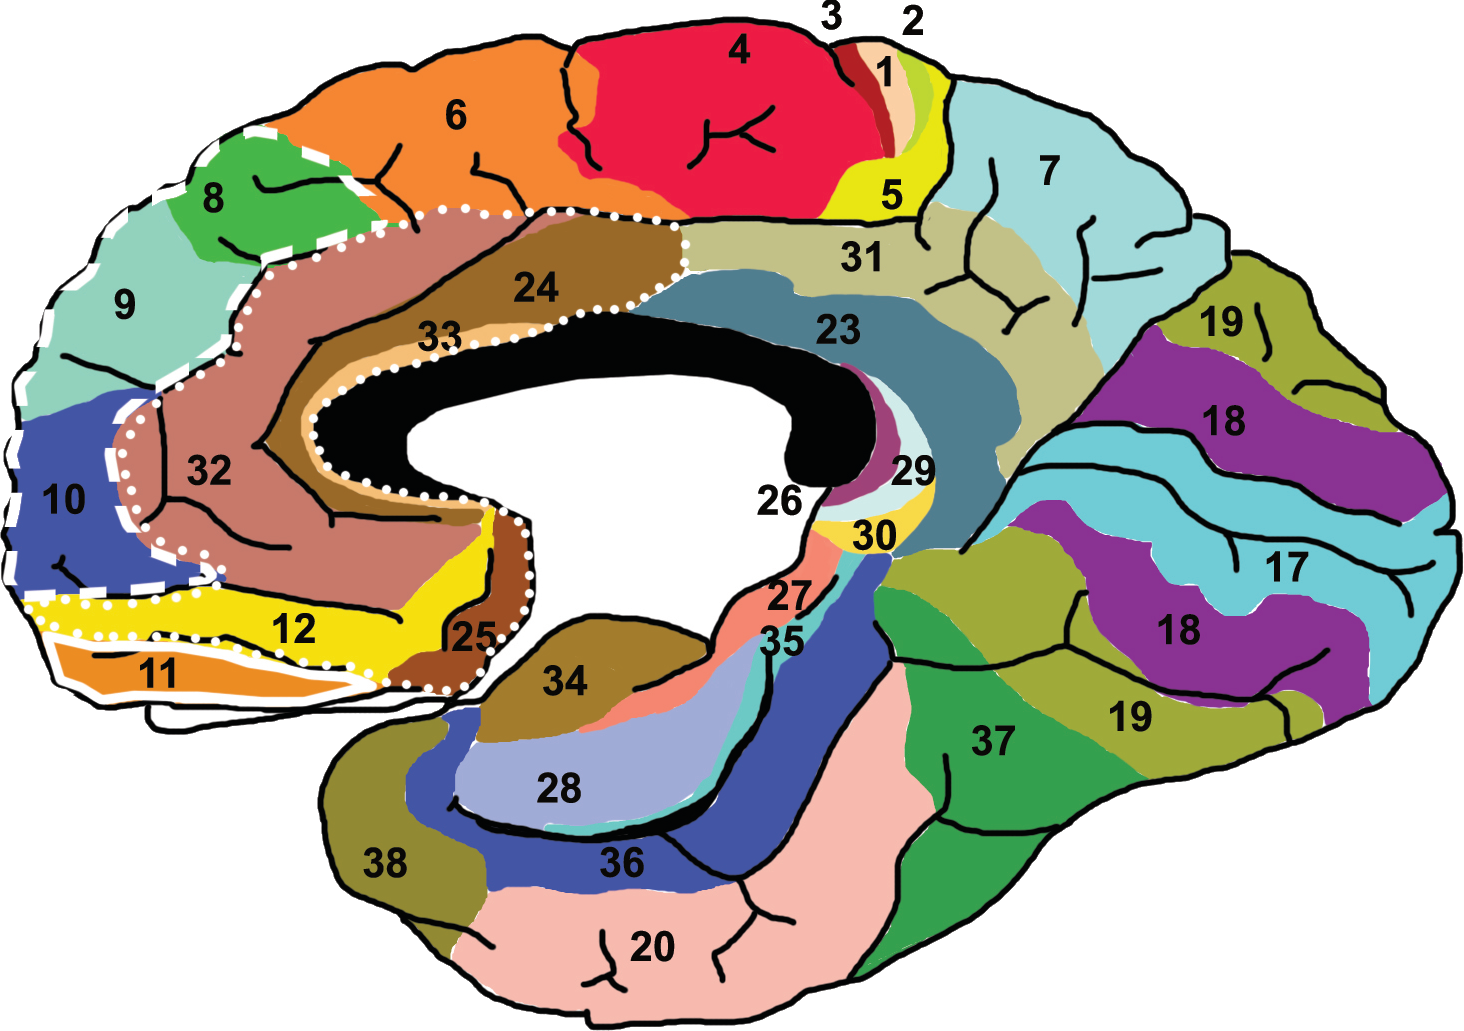
\includegraphics[width=0.8\linewidth]{brodmann_medial}
		\caption{Medial surface}
		\label{fig:brodmann_medial}
	\end{subfigure}
	\caption{Brodmann map of functional partitions.}
	\label{fig:corticalfunctions}
\end{figure}


\begin{itemize}
	\item{Association areas, which are related to perception, memory and thought processes:
		\begin{itemize}
			\item {Prefrontal cortex (areas 8-14,24,25,32,44-47): anterior part of the surface of the frontal lobe. It is centrally involved in cognitive control functions, spanning attention, salience detection, inhibitory control, prospective memory, and cognitive flexibility, as well as long-term pain \. It is one of the least functionally disentangled parts of the cortex \cite{Chini2021}, presenting difficulties in every level of study, with human prefrontal cortex exhibiting a higher relative size, more increased cellular type complexity, more complicated neuronal migration and denser connectivity patterns than other animals. 
				
				
				Experiments have shown that a series of important cognitive  processes takes place there, including working memory (i.e. short-term temporarily stored memory, related to a certain task), attention, salience detection and inhibitory control, related to the ability of adaptation to variable tasks. }
			\item {Inferotemporal cortex (areas 20,21,37)}
			\item {Posterior parietal cortex (areas 5,7)}
		\end{itemize}}
	\item{Sensory areas:
	\begin{itemize}
		\item {Somatosensory cortex (areas 1-3)}
		\item {Visual cortex (areas 17-19)}
		\item {Auditory cortex (areas 41,42)}
		\item {Gustatory cortex (area 43)}
	\end{itemize}}
	\item{Motor areas:
	\begin{itemize}
			\item {Premotor and supplementary motor area cortex (area 6)}
			\item {Primary motor cortex (area 4)}
	\end{itemize}}	
	
\end{itemize}




 In later years, with the advance of imaging methods, new maps have been manufactured, to automatically partition the extracted \ac{3d} cortical projection, based on morphological characteristics. One such gyral-based atlas, \ac{dk}, is derived from the changes in curvature under an expert-driven model of gyri locations \cite{Desikan2006} and provides automatic \textbf{cortical parcellation}. TO BE CONTINUED




\section{Genetic studies on cerebral symmetry}






\section{Phenotypic trait analysis}\label{sec:phenotype_intro}
\subsection{Summary on cortex anatomy}
 
\subsection{Dataset Description}
 
\subsection{Shapes Normalization}
\Ac{mri} output is affected by the subject positioning and technical error.  Volumetric differences also increase the level of discrepancies among \ac{mri} samples. To prevent positioning and volume deviations from gravely affecting shape comparisons, a normalization is required, achieved by projecting each subject onto \textbf{Kendall shape space} \cite{Klingenberg2020}. TO BE CONTINUED

 
\subsection{Asymmetry Components}
TO BE CONTINUED
Of primary interest in this work is \ac{da}, the asymmetric component that arises by comparing a single individual's hemispheric surfaces landmarks differences, computed through a process of alignment, reflection and subtraction of the landmarks pairs. \ac{da} captures information about anatomic characteristics, such as the overall counterclockwise torque, named `Yakovlevian torque' \cite{LeMay1976}, that is observed in humans between the right and left hemisphere (\autoref{fig:yaktorque}). Past studies have shown that abnormal \ac{da} may be an indication of certain diseases. The lack of it may imply schizophrenia predisposition \cite{Ribolsi2014}. Any significant abnormalities may be indicative of other psychiatric disorders, such as autism or developmental language disorder \cite{Herbert2005}\cite{Kong2022}. 

\subsubsection{Statistical analysis}
Bilateral asymmetry is mainly described using three components in literature \cite{klingenberg2002}\cite{Vingerhoets2021}; \acf{da}, the focus of this study, corresponds to the hemispheric side effect; antisymmetry, which is related to the effect where sidedness is random in a population (i.e. left-right randomly switches to right-left), is not observed in the human cerebral cortex, in contrast to other internal organs positions, or organisms \cite{Neubauer2020}; \acf{fa}, encompasses any random developmental and environmental effects, that cannot be explained with the existing knowledge. The observed deviations can be statistically linearly modeled as products of two effects, the hemisphere side studied and the individual specimen analyzed, as well as their interaction \cite{klingenberg2002}. Formally, based on \cite{VanDongen1999} assuming the presence of replications of the observation per individual, to account for technical error, a mixed linear model representing the aforementioned dependencies is defined as:
\begin{equation}
	Y_{ijk} = \mu + \beta + I_i + S_{ij} + E_{ijk}
\end{equation}
where $Y_{ijk}$ is the phenotype of the i-th individual, from the j-th side, under the k-th replication, $\mu$ and $\beta$ are the fixed intercept and fixed side effect respectively, $I_i\sim\mathcal{N}(0,\sigma^2_{ind})$ is the random individual effect,  $S_{ij}\sim\mathcal{N}(0,\sigma^2_{FA})$ is the random side and individual specific effect, matched to \ac{fa}, and $E_{ijk}\sim\mathcal{N}(0,\sigma^2_{ME})$ is the measurement error. Replications are necessary in such a study, in order to differentiate \ac{fa} effect from the measurement error. Given this definition, a way to measure the statistical significance is through an F-test applied on 2-way \ac{anova}, to relate the \ac{rss} ratios of effects to observable error terms, and of fluctuating effect to the measurement error. Extra care needs to be given on the determination of the \ac{dof} of each term, given the preprocessing applied to bring the hemispheres surfaces into Kendall shape space. Those are extracted from the rigorous work in \cite{klingenberg2002}. Given that the analysis is performed on a pair of symmetric objects, and not on a single symmetric object, this configuration is named matching asymmetry analysis. In order to avoid further explicit assumptions, regarding the distribution of TO BE CONTINUED
\subsection{Phenotypic partitioning}\label{sec:hsc}
\Acf{hsc} is an unsupervised method of iterative partitioning, that makes use of the distance matrix eigenvectors \cite{Ng2002}. It results into a binary tree structure (i.e. each parent shape is partitioned into two children). In the current study, a level-4 partitioning is performed, resulting into 31 partitions. Subsequently, they are transformed to the corresponding principal components that explain 80\% of the variance, for reasons of further dimensionality reduction. TO BE CONTINUED


\begin{figure}
	\centering
	\includesvg[]{torque0510}
	\caption[Yakovlevian torque]{Illustration of the Yakovlevian torque. Displayed by a red line rotated counterclockwise 0.51 degrees in relation to the perfectly vertical black line, as calculated by using the average angle of the longest edges (in blue) of the convex hulls of the horizontal plane projection of each hemisphere midthickness surface, after a scaling and alignment process, across the studied population.}
	\label{fig:yaktorque}
\end{figure}

\section{Breaking the complexity into parts}
TO BE EXPANDED

The present work evaluates the brain asymmetry genetic landscape in a coarse-to-fine segmentation, through the application of \ac{hsc}\cite{Ng2002}, discussed in \autoref{sec:hsc}. The technique has been used in a number of different related studies \cite{Claes2018}\cite{Naqvi2021}, yielding results that are in accordance with the underlying anatomic features. The main reason behind this partitioning is the intrinsic complexity of the studied phenotype, eliciting expected differences in the genomic profiles of each cerebral cortex region. The basic assumption made is that topologically close landmarks share similar genetic background. In general though, this type of distance-based clustering is governed by the least quantity of assumptions, regarding the shape or form of the cluster \cite{VonLuxburg2007}. The partitions' genetic juxtaposition is valuable for identifying which regions share similar significant genetic loci, highlighting the corresponding genes contribution, or showcasing the specialization of certain regions that share little to no similarities with their neighbors. Identifying the latter provides a way of mapping the developmental activation of each locus, bringing forth the opportunity to augment the results of related developmental studies \cite{Vijayakumar2016}.

\section{Searching for the origin}
TO BE EXPANDED

The genomic studies are performed under the framework of \ac{snp}-by-\ac{snp} \ac{cca}. The goal is to incorporate multi-allelic \acsp{snp} and, more importantly, multivariate phenotype, in a single hypothesis test per \ac{snp}, that is whether the phenotype is significantly correlated with each analyzed \ac{snp}. In general, there is an abundance of strategies on how to perform multivariate \ac{gwas}, ranging from direct methods, that approximate the inputs relation either in an unbiased manner or making certain educated guesses, to more complex techniques, that increase statistical power by transforming the inputs, at the expense of explanatory ability \cite{Galesloot2014}. There are also methods that are based on the meta-analysis of outcomes from univariate studies, commonly used to juxtapose experiments from separate sources, for which the original data is absent or the exact replication of the study is arduous \cite{Cichonska2016}. Which approach performs best mainly lies on the dataset properties and the nature of the scientific question. Factors such as low sample size \cite{Sheng2021}, genes pleiotropic effects \cite{Fernandes2021} or within-study variation \cite{Jackson2011} tend to handicap the statistical modeling and increase the type I and II errors of the corresponding hypothesis tests. In this study, \ac{cca} was primarily chosen due to the high capacity in efficiently reducing the inputs dimensionality while preserving most information regarding their correlation. Diverse experiments, analyzed in \autoref{chap:gwas}, have been applied to identify the method that gives high fidelity results, consistent with relevant literature. The analysis outcome requires further processing, as explained in \autoref{sec:postprocessing}, to account for the main weakness of this method, that it does not consider the \ac{snp}-to-\ac{snp} effect, tackled using as proxy the notion of \ac{ld}, and subsequently to topologically and functionally enhance the filtered findings. Once this additional step has been performed, a cross-traits analysis is applied, described in \autoref{sec:metaanalysis}, where the \ac{da} genetic signature is compared with the signatures of phenotypic traits, analyzed in a similar study \cite{Naqvi2021}, the cerebral and facial shapes.


\section{Data description}
In this study, targeted on humans, a cross section between the dependent cerebral asymmetry and the independent genetic factors is performed, in an effort to discover affiliated genetic regions and provide a novel understanding of the related genes cooperation. With the advent of technology capable to collect and process genomes from different individuals in relatively high speed, vast databases have been constructed. One of the main players in the data collection has been UK Biobank; a large-scale database from a randomized consortium of 500,000 individuals, whose genome has been collected, from whom  48,000 subjects had also participated in brain \ac{mri} collection process, as of December 2020 \cite{Littlejohns2020}. In this thesis, we exploit this newly acquired dataset to identify the key loci that are related to the human brain surface symmetry. Only healthy self-proclaimed white European individuals were considered. 

\section{Novelties based on related literature} 
 Due to the biological importance of cerebral bilateral asymmetry, it is a subject that has been rigorously studied from multiple viewpoints.
 \subsection{Evolution}
 From an evolutionary stand, it is extremely rare for the right conditions to occur, in order for any soft tissue specimen to be preserved, across a considerable amount of time. The only known way is through mineralization \cite{Purnell2018}. This fact renders a mammal's ancestor brain almost impossible to retrieve. Nevertheless, endocranial imprints have been used as a proxy to describe the relationships between hominids and their ancestors \cite{Balzeau2012}\cite{Neubauer2020}. The reason behind this phenotypic delegation is purely practical. The brain size and shape follow the container volume restrictions. Although such studies support the theory of propagating asymmetry among studied individuals, with the most evident signs of \ac{da} in human skulls, little information about the surface shape can be retrieved, as only the convex hull shape of the brain can be delineated from such process. Through the association of brain asymmetry with \acs{dna}, a universal code among organisms, it becomes possible to deploy tools used by evolutionary geneticists, to identify the phylogenetic tree of this complex trait, locating conserved regions among organisms and their predicted divergence in time, under a pleiotropic model \cite{Koch2021}.
 \subsection{Clinical studies}
 